\chapter{Teoria rozpoznawania mówcy}\label{chap:teoria}

\section{Przetwarzanie mowy}\label{sec:przetwarzanie_mowy}

\subsection{Współczynniki mel-cepstralne}\label{sec:mfcc}

Współczynniki mel-cepstralne (\shortcut{MFCC}, \foreign{Mel Frequency Cepstral Coefficients}),
obok blisko z~nimi związanych \foreign{filter banks} stanowią popularny zestaw
cech dla systemów rozpoznawania mowy i~rozpoznawania mówcy. Systemy bazujące na głębokich sieciach
neuronowych wykorzystują często nieprzetworzone dalej widmo sygnału (\foreign{spectrum}), gdyż obowiązuje
w nich podejście, by zamiast ręcznie przetwarzać wejście lepiej zapewnić sieci neuronowej
architekturę pozwalającą na nauczenie się odpowiednich cech. Na przykład zamiast ręcznie
projektować filtr lepiej dodać do sieci warstwę konwolucyjną. Bardziej tradycyjne metody
oparte o~\shortcut{GMM} jednak bardzo korzystają na zredukowaniu wymiarowości problemu
oraz zapewnieniu, że poszczególne cechy są nieskorelowane, co zachodzi przy \shortcut{MFCC}.

Krokiem wstępnym policzenia \shortcut{MFCC} jest pre-emfaza (\foreign{preemphasis}), czyli przefiltrowanie sygnału
prostym filtrem górnoprzepustowym, zwykle postaci wektora o~współczynnikach $[-0.95\ 1.0]$ lub \\ $[-0.97\ 1.0]$.
Jak pokazuje rysunek \ref{fig:2_1_b_example_preemphasis}, energia w~wyższych pasmach po tej operacji,
choć początkowo znacznie niższa, została wyrównana z~energią w~niższych pasmach częstotliwości.
Ogranicza to błędy numeryczne
pojawiające się przy dalszym przetwarzaniu, co miało duże znaczenie w~starszych komputerach.

\begin{figure}[H]
    \centering
    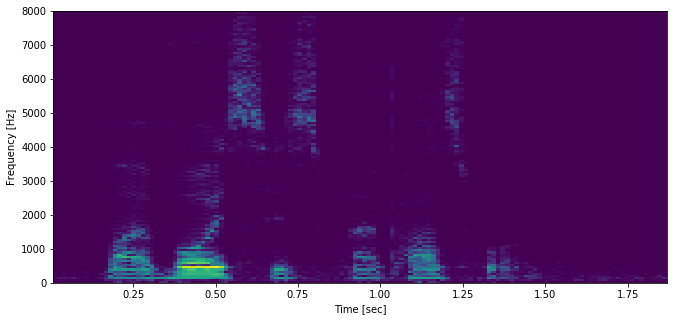
\includegraphics[width=0.8\textwidth]{images/2_1_a_example_spectrogram}
    \caption{Spektrogram sygnału \code{m0002/20150713085938321\underscore m0002\underscore 31.pcm} ze zbioru \techname{RedDots}}
    \label{fig:2_1_a_example_spectrogram}
\end{figure}

\begin{figure}[H]
    \centering
    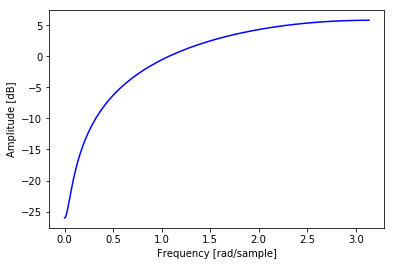
\includegraphics[width=0.6\textwidth]{images/2_1_c_preemphasis_response}
    \caption{Charakterystyka częstotliwościowa filtru typu \foreign{preemphasis} o~współczynnikach $[-0.95, 1.0]$}
    \label{fig:2_1_c_preemphasis_response}
\end{figure}

\begin{figure}[H]
    \centering
    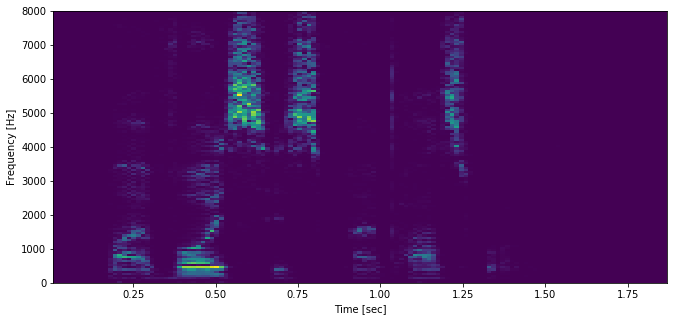
\includegraphics[width=0.8\textwidth]{images/2_1_b_example_preemphasis}
    \caption{Spektrogram tego samego sygnału poddany \foreign{preemphasis}}
    \label{fig:2_1_b_example_preemphasis}
\end{figure}

W drugim kroku należy policzyć \shortcut{STFT} (\foreign{Short Time Fourier Transform}), to znaczy podzielić
sygnał na ramki i~dla każdej ramki policzyć spektrum częstotliwościowe. Dalsze operacje
będą wykonywane na reprezentacji sygnału w~dziedzinie częstotliwości. Typowa szerokość
okna to $25$ms, przy czym każde kolejne okno jest przesunięte o~ok. połowę szerokości,
np. można przyjąć $10$ms. W~przypadku zbioru \techname{RedDots} nagrania mają częstotliwość próbkowania $16$kHz,
więc by uzyskać takie przesunięcie okna muszą zawierać $400$ próbek z~przesunięciem $160$ próbek.
Następnie spektra zamieniane są w~spektra mocy przez wzięcie kwadratu wartości absolutnej
z każdej wartości w~spektrum.

Wynik \shortcut{STFT} można zwizualizować jako spektrogram, jak na rysunku \ref{fig:2_1_a_example_spectrogram},
i zawiera on informacje o~tym jak energia sygnału w~różnych pasmach zmieniała się w~czasie.
Każde okno można wyciąć z~użyciem okna Hamminga lub Hanna, które mają mniejszy wpływ
na wynikowe spektrum sygnału niż okno prostokątne (wycięcie wybranego przedziału próbek
z sygnału jest równoważne przemnożeniu przez okno prostokątne)

Następnie budowany jest bank filtrów w~skali melowej. Przeliczenia częstotliwości w~melach na
częstotliwość w~Hertzach dokonuje się według poniższych wzorów.
$$m = 2595 log_{10}(1 + \frac{f}{700})$$
$$f = 700 (10^{m/2595} - 1)$$
Jest to skala w~nieliniowej zależności z~Hertzami. Jej postać i~stałe zostały tak dobrane,
że zmiana w~tej skali odpowiada subiektywnemu odczuciu zmiany wysokości dźwięku przez ludzi.

Bank filtrów składa się z~pewnej liczby, zwykle $20$ lub $26$, trójkątnych filtrów o~równej
szerokości w~skali melowej, rozmieszczonych z~przesunięciem 50\% szerokości. Ich szerokość
jest tak dobrana, by pokryły cały przedział częstotliwości sygnału.

\begin{figure}[H]
    \centering
    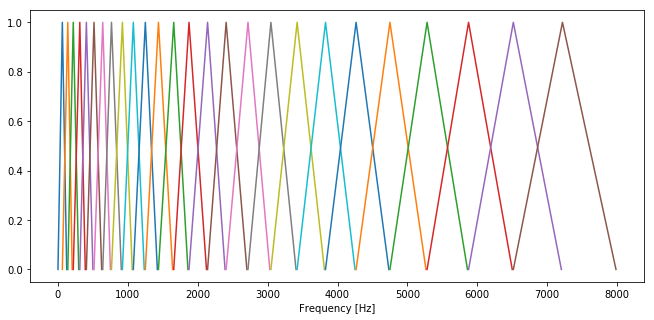
\includegraphics[width=0.8\textwidth]{images/2_1_d_mel_filters}
    \caption{Charakterystyka w~skali Hertza banku 20 trójkątnych filtrów o~równej szerokości w~skali melowej}
    \label{fig:2_1_d_mel_filters}
\end{figure}

Mając te filtry następnym etapem przetwarzania sygnału jest przemnożenie widma przez każdy z~tych filtrów i~zsumowanie
dzięki czemu uzyskuje się jedną liczbę na filtr - całkowitą energię sygnału na pokrytych filtrami pasmach.

Uzyskane sumy są następnie logarytmowane. Pozwala to na dekonwolucję sygnału mowy i~wpływu środowiska.
Dekonwolucja przebiega w~ten sposób, że najpierw dzięki policzeniu transformaty Fouriera,
uzyskiwane jest spektrum, a~konwolucja sygnału w~czasie jest równoważna przemnożeniu widm częstotliwościowych.
Następnie jak ten iloczyn widm zostanie zlogarytmowany, to można go przedstawić jako sumę logarytmów.
W wynikowych cechach jeżeli sygnał mowy został z~czymś spleciony, to skutkuje to tylko przesunięciem cech
ze wszystkich ramek. Można wtedy, przy założeniu, że wpływ otoczenia jest stały, znormalizować średnią tych cech,
by zmniejszyć jego wpływ.

Znormalizowane współczynniki filtrów melowych bywają używane jako gotowy zestaw cech. Do uzyskania \shortcut{MFCC},
widocznej na rysunku \ref{fig:2_1_e_mfcc},
potrzebne jest jeszcze policzenie dyskretnej transformaty cosinusowej (\shortcut{DCT},
\foreign{Discrete Cosine Transform}). Dyskretna transformata cosinusowa to modyfikacja
transformaty Fouriera, która w~wyniku daje ciąg współczynników rzeczywistych, a~nie zespolonych. Wykorzystana jest
właściwość \shortcut{DFT} (\foreign{Discrete Fourier Transform}), że jeżeli sygnał w~dziedzinie czasu ma
współczynniki rzeczywiste, to współczynniki transformaty
będą cechować się symetrią sprzężoną. A~jeżeli sygnał w~dziedzinie czasu jest symetryczny,
to transformata będzie miała tylko współczynniki rzeczywiste. \shortcut{DCT}
(\foreign{Discrete Cosine Transform}) liczy się zatem tak,
iż tworzony jest nowy sygnał dwa razy większej długości niż
sygnał wyjściowy, przez odbicie wyjściowego sygnału. Taki sygnał będzie symetryczny i~rzeczywisty, więc jego transformata
Fouriera będzie również symetryczna i~rzeczywista. Połowę transformaty można odrzucić, a~druga połowa, zawierająca
współczynniki rzeczywiste i~będąca takiego samego rozmiaru co wyjściowy sygnał, nazywamy dyskretną transformatą cosinusową.

Fakt, że \shortcut{DCT} sygnału jest również rzeczywista i~ma ten sam rozmiar jest wygodny, lecz liczy się
ją przede wszystkim dlatego, że ma właściwości dekorelacyjne. Zademonstrowano to na rysunkach
\ref{fig:2_1_f_correlation_matrix_banks} i~\ref{fig:2_1_g_correlation_matrix_mfcc}.
Dzięki temu przy modelowaniu \shortcut{MFCC} za pomocą wielowymiarowej
dystrybucji normalnej można przyjąć, że
współczynniki są nieskorelowane i~zastosować uproszczenie, że macierz kowariancji parametryzująca tę dystrybucję
jest macierzą diagonalną.

\begin{figure}[H]
    \centering
    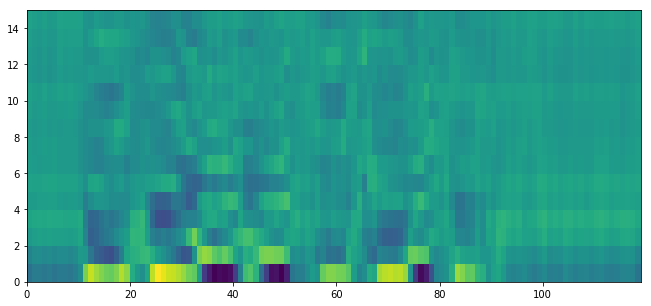
\includegraphics[width=0.8\textwidth]{images/2_1_e_mfcc}
    \caption{Wizualizacja 15 pierwszych współczynników \shortcut{MFCC} dla każdej ramki przykładowego sygnału}
    \label{fig:2_1_e_mfcc}
\end{figure}

Współczynniki wyjściowe \shortcut{DCT} określamy jako współczynniki mel-cepstralne i~ze względu na
wspomniane właściwości użyjemy ich
w naszych systemach. W~praktyce z~$26$ współczynników wybiera się tylko pierwsze $13$ lub $20$, gdyż dalsze opisują
wysokie częstotliwości kształtu widma, które są nieprzydatne przy rozumieniu sygnału mowy.
Do tych współczynników dołącza się $26$ lub $40$
współczynników delta oraz delta-delta, obliczonych jako różnica między wartościami współczynników w~obecnej i~poprzedniej
ramce. Współczynniki delta opisują jak konkretne współczynniki zmieniają się w~czasie,
choć zapewne tracą na przydatności w~modelach jak sieci neuronowe, które mogą na wejściu przyjąć nie tylko jedną ramkę sygnału,
ale też kilka sąsiadujących ramek.

\begin{figure}[H]
    \centering
    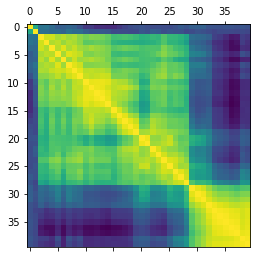
\includegraphics[width=0.6\textwidth]{images/2_1_f_correlation_matrix_banks}
    \caption{Macierz korelacji dla współczynników uzyskanych z~banku filtrów}
    \label{fig:2_1_f_correlation_matrix_banks}
\end{figure}

\begin{figure}[H]
    \centering
    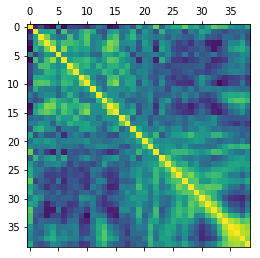
\includegraphics[width=0.6\textwidth]{images/2_1_g_correlation_matrix_mfcc}
    \caption{Macierz korelacji dla współczynników \shortcut{MFCC}}
    \label{fig:2_1_g_correlation_matrix_mfcc}
\end{figure}

\subsection{Mikstury gaussowskie}\label{sec:gmm}

Mikstura rozkładów to sposób opisu rozkładu zmiennej losowej $X$ przez wprowadzenie dodatkowej ukrytej zmiennej $\Theta$.
Następnie uznaje się, że dla każdej wartości zmiennej ukrytej rozkład zmiennej pochodzi z~innego rozkładu.
Zwykle zmienna ukryta jest dyskretna, wyjściowa zmienna może być dyskretna lub ciągła i~przyjmuje się, że wszystkie
warunkowe rozkłady $P(X|\Theta)$ pochodzą z~tej samej rodziny i~różnią się parametrami. Rozkład zmiennej $X$ można
uzyskać przez marginalizację zmiennej ukrytej.
$$f(x) = \sum_{\theta_i} f(X | \theta_i) P(\theta_i)$$
Przy miksturach gaussowskich (\shortcut{GMM}, \foreign{Gaussian Mixture Model}) przyjmuje się, że warunkowe prawdopodobieństwa zmiennej wyjściowej od zmiennej ukrytej
należą do rodziny wielowymiarowych rozkładów normalnych, tj. mają gęstość
$$f(x | \theta_i) = \frac{1}{\sqrt{(2 \pi)^d |\Sigma_i|}} \exp(-\frac{1}{2} (x - \mu_i)^T \Sigma_i^{-1} (x - \mu_i))$$
gdzie $\mu_i$ to $d$-wymiarowy wektor średnich, $\Sigma_i$ to macierz kowariancji rozmiaru $d \times d$

\begin{figure}[H]
    \centering
    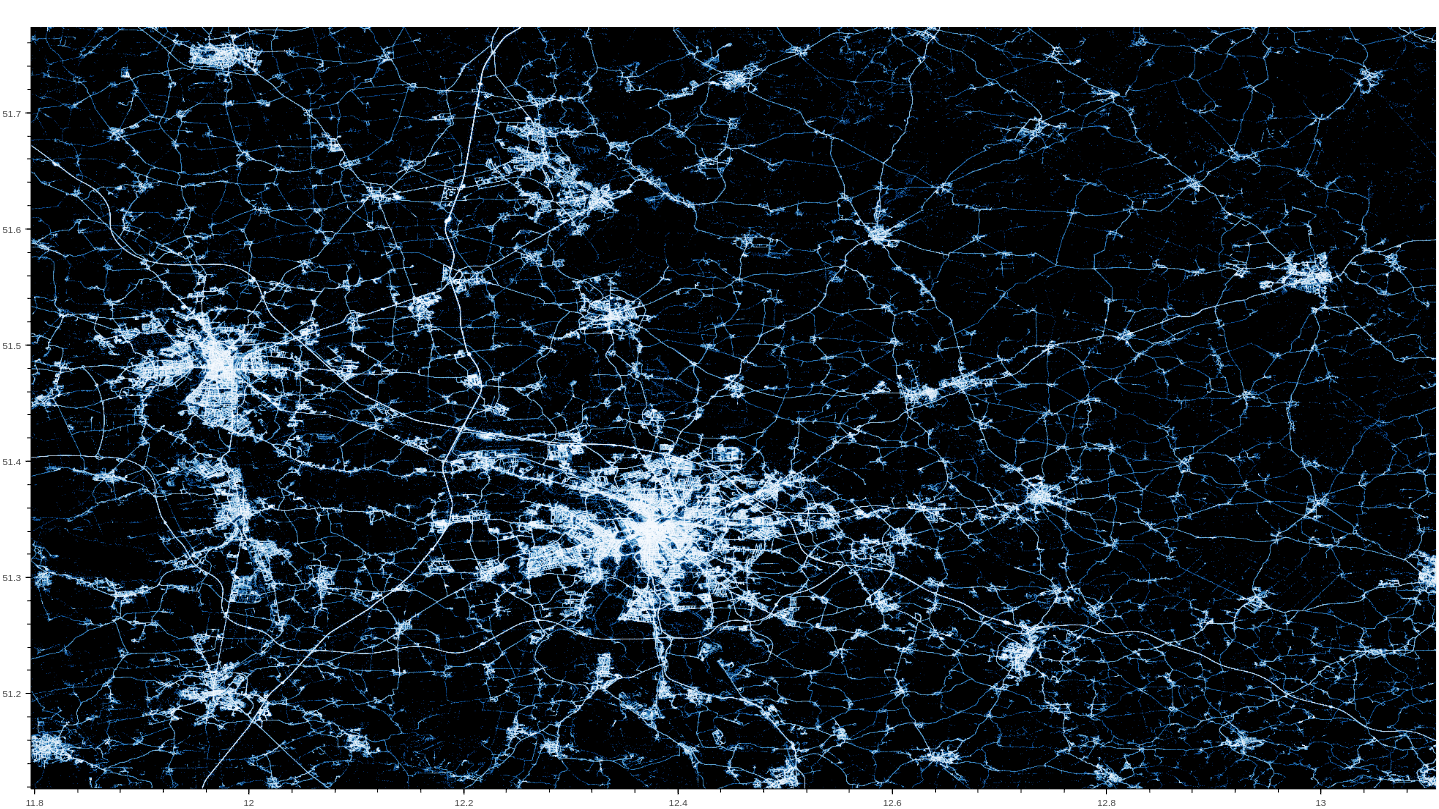
\includegraphics[width=0.9\textwidth]{images/2_2_a_leipzig_datashader}
    \caption{Wizualizacja \foreign{datashader} danych o~przejazdach w~okolicach Lipska pobranych z~nawigacji samochodowych}
    \label{fig:2_2_a_leipzig_datashader}
\end{figure}

\begin{figure}[H]
    \centering
    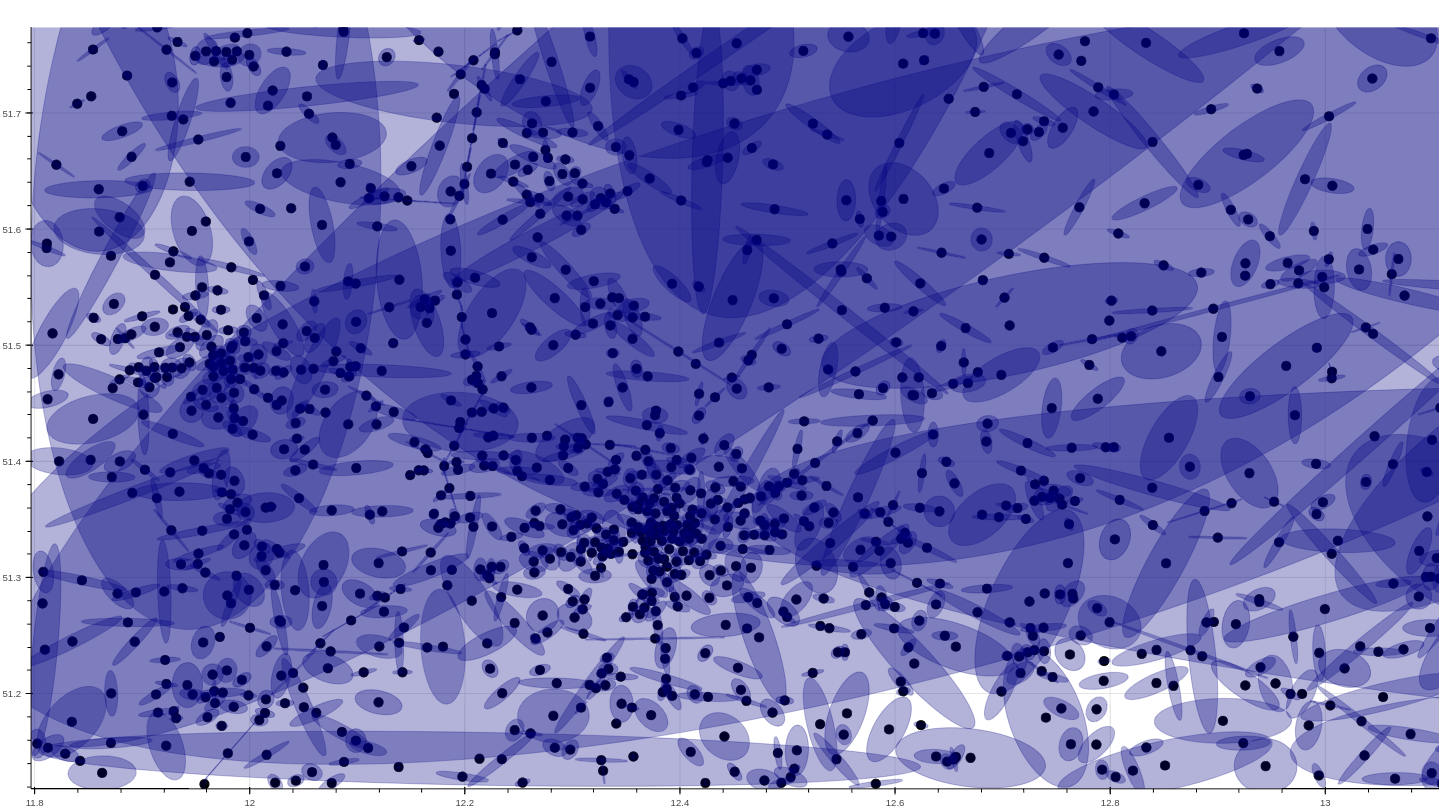
\includegraphics[width=0.9\textwidth]{images/2_2_a_leipzig_gmm}
    \caption{Wizualizacja \shortcut{GMM} dopasowanych za pomocą \shortcut{EM} do danych o~przejazdach z~rysunku \ref{fig:2_2_a_leipzig_datashader}}
    \label{fig:2_2_a_leipzig_gmm}
\end{figure}

Na przykład, na rysunku \ref{fig:2_2_a_leipzig_gmm} zaprezentowano model \shortcut{GMM} dwuwymiarowej dystrybucji,
z której pochodzą punkty z~rysunku \ref{fig:2_2_a_leipzig_datashader}. W~pracy \shortcut{GMM} zostaną wykorzystane
jednak do zamodelowania dystrybucji cech opisujących ramki z~nagrania mowy.

\subsection{Maksymalizowanie wartości oczekiwanej}\label{sec:expectation_maximization}

Parametry wielowymiarowego rozkładu normalnego można wyestymować na podstawie próby, na przykład
stosując estymator maksymalizujący prawdopodobieństwo danych.

Estymatory parametrów maksymalizujące prawdopodobieństwo $M$ elementów $x^j$ to:
$$\hat{\mu} = \frac{1}{m} \sum_{j=0}^M x^{j}$$

$$\hat{\Sigma} = \frac{1}{m} \sum_{j=0}^M (x^{j} - \hat{\mu})^T (x^{j} - \hat{\mu})$$
Jednak w~przypadku mikstury, jeżeli nie przypiszemy z~góry próbek wybranym wartościom ukrytej zmiennej, problem
estymacji parametrów wymaga innego podejścia. Jedną z~metod jest \foreign{Expectation Maximization}, iteracyjny
algorytm wyznaczania wartości parametrów dla mikstur dystrybucji lub ogólniej dla modeli z~ukrytymi zmiennymi.
Składa się z~dwóch kroków wykonywanych na zmianę do uzyskania zbieżności.  Algorytm nie gwarantuje znalezienia
globalnie optymalnego rozwiązania.

\begin{itemize}
    \item \foreign{Expectation} - oszacuj wartości ukrytych parametrów, w~przypadku \shortcut{GMM} przypisz próbom
        prawdopodobieństwo tego, z~jakiej mikstury zostały wygenerowane. Parametry jawne są tutaj niezmieniane,
        ich początkowe wartości można losowo zainicjalizować. Trzeba pamiętać jednak, by cechowały się dużą wariancją
        lub inaczej gwarantowały, że każda z~próbek jest zgodnie z~ich wartościami możliwa do wygenerowania. Inaczej
        pełne dopasowanie do danych będzie niemożliwe. Bardzo małe prawdopodobieństwo może przez błędy numeryczne
        zostać zaokrąglone do $0$ i~również spowodować błąd.
    \item \foreign{Maximization} - zakładając wyznaczone wartości ukrytych parametrów, znaleźć nowe \shortcut{MAP}
        (\foreign{Maximum a~Posteriori}) estymaty
        jawnych parametrów. Trzeba zwrócić uwagę, że pewne mikstury mogą nie mieć przypisanych żadnych próbek
        i~wtedy uaktualnienie parametrów jest niemożliwe. Do tego uaktualniając wagi \shortcut{GMM} należałoby
        przypisać takiej miksturze wagę $0$, przez co nigdy nie byłaby już użyta. Trzeba zwrócić uwagę na ten problem
        i~postarać się o~lepsze zaincjalizowanie parametrów, dodatkowo modyfikować parametry, by nie dopuścić
        do takiej sytuacji lub przynajmniej pamiętać, by usunąć mikstury z~wagą $0$, gdyż będą niepotrzebnie zajmować
        zasoby komputera.
\end{itemize}

\subsection{Dynamic Time Warping (DTW)\cite{ADynamicProgrammingApproach}}\label{sec:dtw}

Jako że praca dotyczy rozpoznawania zależnego od tekstu, konieczne by uzyskać wartościowe wyniki będzie
użycie metod pozwalających na uwzględnienie informacji o~sekwencji ramek. Samo dopasowanie mikstur do ramek
tej informacji nie uwzględni. Jedną z~takich metod jest \foreign{dynamic time warping}.

\shortcut{DTW} to algorytm do porównywania dwóch ciągów. Ciągi mogą być różnej długości i~algorytm zwróci
dla nich wysokie podobieństwo (małą odległość) nawet jeśli pewne podciągi będą bardziej rozciągnięte lub krótsze
w jednym ciągu niż w~drugim.

Algorytm wymaga wybrania metryki (oznaczmy ją $d$) określającej odległość pojedynczych elementów ciągu.
Elementy te mogą być liczbami, ale również wektorami.

\shortcut{DTW} wykorzystuje technikę programowania dynamicznego i~w~podstawowej wersji znanej autorowi wymaga liczby operacji
rzędu $\Theta(n \times m)$, gdzie $n$ i~$m$ to długości porównywanych ciągów oraz ma złożoność pamięciową liniową
względem długości krótszego ciągu. Istnieją jego bardziej wydaje wersje, w~tym wersje z~oknem, tzn. bazujące na
założeniu, że nie ma sensu porównywać elementów z~dwóch ciągów ze zbyt odległymi indeksami.

Algorytm wygląda tak: Na początku inicjalizowana jest macierz odległości $D$ rozmiaru $n + 1 \times m + 1$. Pierwszy
rząd i~pierwsza kolumna jest wypełniana cyfrową reprezentacją $\infty$, co oznacza tyle,
że te wartości nie są brane pod uwagę w~następnym kroku.
Wyjątkiem jest komórka w~pierwszym rzędzie i~pierwszej kolumnie z~wartością $D_{0,0} = 0$.

Pozostałe wartości macierzy są liczone ze wzoru
$$D_{i+1, j+1} = min(D_{i+1, j}, D_{i, j+1}, D_{i, j}) + d(N_i, M_j)$$
gdzie $N_i$ i$M_j$ oznaczają elementy porównywanych ciągów, a~$d(N_i, M_j)$ to jak już wspomniano wybrana
niezależnie od algorytmu odległość między dwoma elementami. Odległość ciągów od siebie znaleziona przez \shortcut{DTW}
to $D_{n, m}$.  Licząc te wartości rzędami możliwe jest osiągnięcie liniowej złożoności pamięciowej względem
długości krótszego ciągu.

Powyższy wzór na $D_{i+1, j+1}$ należy zinterpretować tak, że liczymy odległość pary elementów $N_i$, $M_j$ i~dodajemy
do najbardziej korzystnego wyniku spośród trzech opcji:

\begin{itemize}
    \item Wybór $D_{i+1, j}$ oznacza, że obecny rezultat składa się z~$d(N_i, M_{j-1})$ i~$d(N_i, M_j)$, a~więc ten sam element ciągu $N$ jest porównany z~dwoma elementami ciągu $M$. Na przykład porównując $N = [1, 20, 20, 20, 20]$, $M = [1, 1, 1, 10]$ i~stosując jako miarę odległości różnicę absolutną ten przypadek będzie kilka razy najkorzystniejszy.
    \item Wybór $D_{i, j+1}$ oznacza, że w~sumie będzie zarazem $d(N_{i-1}, M_j)$ i~$d(N_i, M_j)$, a~więc dwa elementy ciągu $N$ są porównane z~tym samym elementem ciągu $M$. Na przykład w~wyniku dla $N = [1, 1, 1, 1, 1, 20]$ i~$ M = [1, 10]$ ten przypadek będzie się składał na wynik minimalizujący odległość ciągów.
    \item $D_{i, j}$ oznacza, że obliczono odległość następnego elementu zarówno z~ciągu $N$ i~z ciągu $M$. Przy porównywaniu $N = [1, 2, 3, 4]$ oraz $M = [1, 2, 3, 4]$ zajdzie wyłącznie ten przypadek.
\end{itemize}

Poniżej przedstawiono kilka przykładów tabelek z~wynikami $DTW$. Elementami są liczby, a~w~roli metryki jest moduł różnicy.

\begin{table}[H]
    \caption{Macierz $D$ dla $DTW$ na dwóch przykładowych sekwencjach $N$ i~$M$. Przykład gdy elementy jednej sekwencji są wielokrotnie dopasowane do pierwszego elementu z~drugiej sekwencji, dopóki jest to możliwe}
    \centering
    \label{tab:dtw_example0}
    \small
    \tabulinesep =_3pt^3pt
    \begin{tabu}{r*{7}{r}}
        \multirow{2}{*}{} & & \multicolumn{5}{c}{N}
        \\
        & & - & 1 & 20 & 20 & 20 & 20
        \\ \midrule
        \multirow{5}{*}{M} & - & 0 & $\infty$ & $\infty$ & $\infty$ & $\infty$ & $\infty$
        \\
        & 1 & $\infty$ & 0 & 19 & 38 & 57 & 76
        \\
        & 1 & $\infty$ & 0 & 19 & 38 & 57 & 76
        \\
        & 1 & $\infty$ & 0 & 19 & 38 & 57 & 76
        \\
        & 10 & $\infty$ & 9 & 10 & 20 & 30 & \textbf{40}
        \\
    \end{tabu}
\end{table}

\begin{table}[H]
    \caption{Macierz $D$ dla $DTW$ na dwóch przykładowych sekwencjach $N$ i~$M$. Przykład z~dokładnie dopasowanymi sekwencjami, z~wydłużonymi lub skróconymi fragmentami}
    \centering
    \label{tab:dtw_example1}
    \small
    \tabulinesep =_3pt^3pt
    \begin{tabu}{r*{11}{r}}
        \multirow{2}{*}{} & & \multicolumn{9}{c}{N}
        \\
        & & - & 1 & 1 & 2 & 3 & 3 & 3 & 4 & 4
        \\ \midrule
        \multirow{7}{*}{M} & - & 0 & $\infty$ & $\infty$ & $\infty$ & $\infty$ & $\infty$ & $\infty$ & $\infty$ & $\infty$
        \\
        & 1 & $\infty$ & 0 & 0 & 1 & 3 & 5 & 7 & 10 & 13
        \\
        & 2 & $\infty$ & 1 & 1 & 0 & 1 & 2 & 3 & 5 & 7
        \\
        & 2 & $\infty$ & 2 & 2 & 0 & 1 & 2 & 3 & 5 & 7
        \\
        & 2 & $\infty$ & 3 & 3 & 0 & 1 & 2 & 3 & 5 & 7
        \\
        & 3 & $\infty$ & 5 & 5 & 1 & 0 & 0 & 0 & 1 & 2
        \\
        & 4 & $\infty$ & 8 & 8 & 3 & 1 & 1 & 1 & 0 & \textbf{0}
        \\
    \end{tabu}
\end{table}

\subsection{Ukryte modele Markowa}\label{sec:hmm}

Ukryty model Markowa (\shortcut{HMM}, \foreign{Hidden Markov Model}) to proces stochastyczny,
dyskretny w~czasie, pozwalający na modelowanie dystrybucji
sekwencji zdarzeń. Będzie zatem użyteczny ze względu na możliwość uwzględnienia w~nim zależności
między ramkami w~czasie.

Model składa się ze zbioru $N$ ukrytych stanów $X = \{x_0, x_1, \dots\, x_{N-1}\}$, ciągu zmiennych losowych
$X_t$, $t = 0, 1, \dots, T - 1$ oznaczających ukryty stan w~chwili $t$, rozkładu początkowego stanu ukrytego
$\pi_i = P(X_0 = x_i)$, zbioru obserwacji (emisji, stan jawny) $Y$, przy czym obserwacje mogą być dyskretne
lub ciągłe i~ciągu zmiennych losowych $Y_t$, $t = 0, 1, \dots, T - 1$ określających obserwację w~chwili $t$.

Do tego zdefiniowane są prawdopodobieństwa przejść między stanami oraz rozkłady obserwacji w~każdym stanie.
Kluczową kwestią w~modelu Markowa, zwaną regułą Markowa, jest iż rozkład prawdopodobieństwa następnego stanu $X_t$
zależy wyłącznie od stanu poprzedzającego, nie jest ważna cała historia stanów w~przeszłości. Podobnie rozkład
obserwacji $Y_t$ zależy wyłącznie od obecnego stanu ukrytego.

Inną właściwością, którą się przyjmuje, jest jednorodność. Oznacza to, że przejścia między stanami i~emisje są
niezależne od czasu $t$. Przy dyskretnych i~jednorodnych stanach ukrytych prawdopodobieństwa przejść
między stanami można zapisać w~postaci macierzy $H$ (\foreign{transition matrix}) $P(X_t = x_i | X_{t-1} = x_j) = H_{j, i}$.
Podobnie jeżeli emisje są dyskretne, to można je zapisać w~postaci macierzy $V$ $P(Y_t = y_i | X_t = x_j) = V_{j, i}$.
Lecz emisje często mają jakieś określone parametryczne dystrybucje i~wtedy definiuje się w~postaci wektorów parametrów.
$H$ (oraz $V$ jeżeli mowa o~dyskretnych emisjach) jest macierzą stochastyczną, więc $\forall_{i, j = 0 \dots N - 1} 0 \leq H_{i, j} \leq 1$ i~$\forall_{i = 0 \dots N - 1} \sum_{j = 0}^{N - 1} H_{j, i} = 1$ (wiersze sumują się do 1).

Czasami, w~innych modelach regułę Markowa rozszerza się tak, iż prawdopodobieństwo może zależeć od $k$ ostatnich stanów
$P(X_t | X_{t-1} \dots X_{t-k})$ i~nazywa się to regułą Markowa $k$ rzędu. Są też inne wersje, w~których zbiór
ukrytych stanów jest ciągły, w~których rząd $k$ jest zmienny lub na przykład pola Markowa,
gdzie nie mówimy o~ciągu w~czasie, lecz o~zmiennych rozmieszczonych
w kilku wymiarach, których wartości zależą od pewnego sąsiedztwa. Wszystkie modele Markowa mają jednak cechę wspólną, iż
zmienne losowe zależą w~nich od pewnego skończonej liczby innych zmiennych.

Jeżeli macierz przejść jest tak zdefiniowana, że zawsze możliwe jest przejście z~każdego stanu do każdego, to
mówimy, że model jest ergodyczny. Jednak na przykład w~rozpoznawaniu mowy często definiuje się macierz przejść,
by pozwalała tylko na przejście do stanu o~takim samym lub wyższym indeksie, tzw. model Bakisa lub model lewo-prawo
(\foreign{left-to-right}) albo by miała niezerowe prawdopodobieństwo przejścia wyłącznie z~danego stanu do jego
samego lub stanu o~indeksie o~jeden większym (model \foreign{beads-on-string}).

Ważne w~praktyce jest, że istnieją wydajne algorytmy rozwiązujące następujące problemy \shortcut{HMM}.

\begin{enumerate}
    \item Algorytm w~przód - problem znalezienia prawdopodobieństwa stanu ukrytego w~danej chwili wraz z~pewnym ciągiem obserwacji do tego chwili. Jeżeli tym punktem w~czasie będzie koniec sekwencji obserwacji, to można zmarginalizować prawdopodobieństwo końcowego stanu i~uzyskać prawdopodobieństwo wygenerowania danej sekwencji obserwacji przez model.
    \item Algorytm w~tył - problem znalezienia prawdopodobieństwa ciągu zdarzeń w~przyszłości, pod warunkiem danego stanu ukrytego w~danej chwili. Jest on istotny, gdyż jest częścią następnego algorytmu.
    \item Algorytm w~przód i~w~tył - problem znalezienia prawdopodobieństwa stanu ukrytego w~danej chwili pod warunkiem wystąpienia danego ciągu obserwacji. Brany pod uwagę jest cały ciąg obserwacji, tych przed i~tych po danym stanie ukrytym. Działa przez połączenie wyników algorytmu w~przód i~w~tył, stąd nazwa.
    \item Algorytm Viterbiego - problem znalezienia najbardziej prawdopodobnego ciągu stanów ukrytych dla danego ciągu obserwacji parametrów modelu. Jest podobny do algorytmu w~przód, z~tym, że na każdym kroku wybiera najbardziej prawdopodobną sekwencję zamiast uwzględniać prawdopodobieństwa wszystkich stanów.
    \item Algorytm Bauma-Welcha - problem znalezienia parametrów modelu Markowa (prawdopodobieństwo przejść między stanami ukrytymi, rozkład obserwacji dla każdego stanu ukrytego, rozkład stanu początkowego) maksymalizujących prawdopodobieństwo wystąpienia danego ciągu obserwacji. Wykorzystuje algorytm w~przód i~w~tył oraz opisany wcześniej algorytm \foreign{expectation maximization}, algorytm w~przód i~w~tył służy do wyznaczenia ukrytych zmiennych opisujących jaki był stan w~każdej chwili czasu na potrzeby kroku \foreign{expectation}, a~następnie wyznaczane są najbardziej prawdopodobne parametry emisji w~kroku \foreign{maximization}.
\end{enumerate}

Poniżej wyprowadzono te algorytmy, zakładając przy tym dyskretne emisje.

\subsubsection{Algorytm w~przód}

Algorytm w~przód (\foreign{forward algorithm}) liczy łączone prawdopodobieństwo znalezienia się w~jakimś stanie w~chwili $t$
i wystąpienia pewnego ciągu obserwacji $y_{t-1} \dots y_0$ w~przeszłości. To znaczy oblicza on $P(x_t, y_t \dots y_0)$,
korzystając z~rekurencyjnej zależności:
$$P(x_t, y_t \dots y_0) = \sum_{x_{t-1}} P(x_t, x_{t-1}, y_t \dots y_0) =$$
$$\sum_{x_{t-1}} P(y_t | x_t, x_{t-1}, y_{t-1} \dots y_0) P(x_t | x_{t-1}, y_{t-1} \dots y_0) P(x_{t-1}, y_{t-1} \dots y_0)$$
Dzięki własności Markowa można to uprościć do:
$$P(y_t | x_t, x_{t-1}, y_{t-1} \dots y_0) = P(y_t | x_t) = V_{x_t, y_t}$$
$$P(x_t | x_{t-1}, y_{t-1} \dots y_0) = P(x_t | x_{t-1}) = H_{x_{t-1}, x_t}$$
Ostateczną zależnością jest
$$P(x_t, y_t \dots y_0) = V_{x_t, y_t} \sum_{x_{t-1}} H_{x_{t-1}, x_t} P(x_{t-1}, y_{t-1} \dots y_0)$$
gdzie $P(x_{t-1}, y_{t-1} \dots y_0)$ może być rekurencyjnie obliczone w~ten san sposób aż do przypadku bazowego $P(x_0, \emptyset) = \pi_1$, gdzie $\pi$ to rozkład początkowy.

Użycie własności Markowa pozwala zredukować złożoność obliczeniową problemu z~$\theta(MN^M)$ do $\theta(MN^2)$, gdzie $M$ to możliwa liczba obserwacji, a~$N$ to liczba stanów ukrytych.

\subsubsection{Algorytm w~tył}

Algorytm w~tył (\foreign{backward algorithm}), jest podobny do algorytmu w~przód. Oblicza $P(y_{t+1} \dots y_{T-1} | x_t)$, to znaczy prawdopodobieństwo wystąpienia wskazanej sekwencji obserwacji $y_{t+1} \dots y_{T-1}$, gdzie $T$ to liczba obserwacji, zakładając początkowy stan ukryty $x_t$ w~chwili $t$. Obliczenia zaczyna się od końcowego stanu $x_{T-1}$.
$$P(y_{t+1} \dots y_{T-1} | x_t) = \sum_{x_{t+1}} P(y_{t+1} \dots y_{T-1}, x_{t+1} | x_t) =$$
$$\sum_{x_{t+1}} P(y_{t+1} | y_{t+2} \dots y_{T-1}, x_{t+1}, x_t) P(y_{t+2} \dots y_{T-1} | x_{t+1}, x_t) P(x_{t+1} | x_t)$$
Korzystając z~tego można uprościć:
$$P(y_{t+1} | y_{t+2} \dots y_{T-1}, x_{t+1}, x_t) = P(y_{t+1} | x_{t+1}) = V_{x_{t+1},y_{t+1}}$$
$$P(y_{t+2} \dots y_{T-1} | x_{t+1}, x_t) = P(y_{t+2} \dots y_{T-1} | x_{t+1})$$
$$P(x_{t+1} | x_t) = H_{x_t,x_{t+1}}$$
Ostateczna zależność to:
$$P(y_{t+1} \dots y_{T-1} | x_t) =  \sum_{x_{t+1}} V_{x_{t+1},y_{t+1}} H_{x_t,x_{t+1}} P(y_{t+2} \dots y_{T-1} | x_{t+1})$$
Prawdopodobieństwo jest liczone rekurencyjnie, z~przypadkiem bazowym
$$P(\emptyset | x_{T-1}) = 1$$

\subsubsection{Algorytm w~przód i~w~tył}
Algorytm w~przód i~w~tył (\foreign{forward-backward algorithm}) działa przez połączenie wyników algorytmu w~przód i~w~tył.

Przypomnijmy, że:

\begin{enumerate}
    \item Algorytm w~przód oblicza $P(x_t, y_t \dots y_0)$, to znaczy prawdopodobieństwo dla ukrytego stanu w~chwili $t$ oraz ciągu stanów z~przeszłości.
    \item Algorytm w~tył oblicza $P(y_{T-1} \dots y_{t+1} | x_t)$, czyli warunkowe prawdopodobieństwo ciągu obserwacji z~przyszłości wobec ukrytego stanu w~chwili $t$.
    \item Algorytm w~przód i~w~tył oblicza $P(x_t | y_{T-1} \dots y_0)$. Oblicza zatem prawdopodobieństwo ukrytego stanu $x_t$ w~dowolnej chwili $t$ biorąc pod uwagę cały ciąg obserwacji. Możliwe jest dzięki niemu wybranie najbardziej prawdopodobnego stanu w~każdej chwili. Trzeba zauważyć, że biorąc najbardziej prawdopodobny stan z~każdej chwili niekoniecznie uzyska się najbardziej prawdopodobny ciąg stanów ukrytych odpowiadający ciągowi obserwacji, bo przejście z~jednego bardzo prawdopodobnego stanu do drugiego może być bardzo nieprawdopodobne. Dlatego do tego zadania służy algorytm Viterbiego.
\end{enumerate}

Algorytm \foreign{forward-backward} wykorzystuje poniższe zależności:
$$P(x_t, y_t \dots y_0) P(y_{T-1} \dots y_{t+1} | x_t) = P(y_t \dots y_0 | x_t) P(y_{T-1} \dots y_{t+1} | x_t) P(x_t) = $$
$$P(y_{T-1} \dots y_0 | x_t) P(x_t) = P(y_{T-1} \dots y_0, x_t) = P(x_t | y_{T-1} \dots y_0) P(y_{T-1} \dots y_0)$$
Skąd wynika natychmiast:
$$P(x_t | y_{T-1} \dots y_0) = \frac{P(x_t, y_t \dots y_0) P(y_{T-1} \dots y_{t+1} | x_t)}{P(y_{T-1} \dots y_0)}$$
Prawdopodobieństwa w~liczniku zostały obliczone odpowiednio przez algorytm w~przód i~algorytm w~tył.
Prawdopodobieństwo w~mianowniku można wyznaczyć przez zsumowanie po możliwych wartościach $X_{T-1}$ w~wynikach algorytmu
w przód $\sum_{x_{T-1}} P(x_{T-1}, y_{T-1} \dots y_0)$

\subsubsection{Algorytm Bauma-Welcha}

Algorytm Bauma-Welcha (\foreign{Baum-Welch algorithm}) pozwala na znalezienie najbardziej prawdopodobnych parametrów
$H$, $\pi$, $V$ modelu Markowa zależnie od ciągu obserwacji. Algorytm bazuje na metodzie
\foreign{expectation-maximization}. Wykorzystuje przy tym algorytm w~przód i~w~tył (\foreign{forward-backward})
do znalezienia w~kroku \foreign{expectation} prawdopodobieństw ukrytych stanów dla danej sekwencji obserwacji.
W kroku \foreign{maximization} estymuje parametry szukając takich, które maksymalizują prawdopodobieństwo wystąpienia
obserwacji, przy założeniu takich ukrytych stanów jak to wyznaczono w~poprzednim kroku. Operacje te są powtarzane.

Jak pokazano powyżej, algorytm \foreign{forward-backward} pozwala obliczyć $P(x_t | y_{T-1} \dots y_0)$,
łącząc $P(x_t, y_t \dots y_0)$ $P(y_{T-1} \dots y_{t+1} | x_t)$ liczone przez algorytmy \foreign{forward} i~\foreign{backward}.

Do przeprowadzenia treningu \foreign{Bauma-Welcha} potrzebne jest dodatkowo wyznaczenie $P(x_t, x_{t+1} | y_{T-1} \dots y_0)$,
czyli prawdopodobieństwa przejścia z~jednego stanu w~chwili $t$ do drugiego w~chwili $t + 1$,
uwzględniając sekwencję $T$ obserwacji i, niejawnie, parametrów modelu.
$$P(x_t, x_{t+1} | y_{T-1} \dots y_0)
= \frac{P(x_t, x_{t+1}, y_{T-1} \dots y_0)}{P(y_{T-1} \dots y_0)}$$

$$P(x_t, x_{t+1}, y_{T-1} \dots y_0) = P(y_{T-1} \dots y_0 | x_t, x_{t+1}) P(x_{t+1} | x_t) P(x_t) = $$
$$P(y_{T-1} \dots y_{t+2} | x_t, x_{t+1}) P(y_{t+1} \dots y_0 | x_t, x_{t+1}) P(x_{t+1} | x_t) P(x_t)$$

Iloczyn drugiego i~czwartego czynnika możemy wyrazić następująco:
$$P(y_{t+1} \dots y_0 | x_t, x_{t+1}) P(x_t) = P(y_{t+1} \dots y_0, x_t | x_{t+1}) = $$
$$P(y_{t+1} | x_{t+1}) P(y_t \dots y_0, x_t | x_{t+1})$$

Licznik wyrażenia w~pierwszej linijce, korzystając z~wyprowadzonej właśnie zależności oraz z~reguły Markowa o~tym,
iż stan ukryty zależy tylko od poprzedniego stanu, a~emisja zależy od obecnego stanu, można wyrazić tak:
$$P(x_t, x_{t+1}, y_{T-1} \dots y_0) =$$
$$P(y_{T-1} \dots y_{t+2} | x_t, x_{t+1}) P(y_{t+1} | x_{t+1}) P(y_t \dots y_0, x_t | x_{t+1}) P(x_{t+1} | x_t) =$$
$$P(y_{T-1} \dots y_{t+2} | x_{t+1}) P(y_{t+1} | x_{t+1}) P(y_t \dots y_0, x_t) P(x_{t+1} | x_t)$$

$$P(x_t, x_{t+1} | y_{T-1} \dots y_0)
= \frac{P(y_{T-1} \dots y_{t+2} | x_{t+1}) P(y_t \dots y_0, x_t) V_{x_{t+1}, y_{t+1}} H_{x_t, x_{t+1}}}{P(y_{T-1} \dots y_0)}$$
Analogicznie jak w~przypadku algorytmu w~przód i~w~tył, pierwszy czynnik w~liczniku można obliczyć za pomocą
algorytmu w~tył, a~drugi za pomocą algorytmu w~przód. Wtedy można uaktualniać parametry w~poniższy sposób:
$$\pi_i = P(X_0 = x_i | y_{T-1} \dots y_0)$$

$$H_{x_t, x_{t+1}} = \frac{\sum_{t=0}^{T-1} P(x_t, x_{t+1} | y_{T-1} \dots y_0)}{\sum_{t=0}^{T-1} P(x_t | y_{T-1} \dots y_0)}$$

$$V_{x_t, y_t} = \frac{\sum_{t=0}^{T-1} 1_{Y_t = y_t} P(x_t | y_{T-1} \dots y_0)}{\sum_{t=1}^T P(x_t | y_{T-1} \dots y_0)}$$
Założone jest tutaj, iż obserwacje są  dyskretne i~opisane macierzą stochastyczną. W~przeciwnym razie trzeba użyć innego estymatora.
\subsubsection{Algorytm Viterbiego}

Używając algorytmu \foreign{forward-backward} można obliczyć prawdopodobieństwa dla każdego stanu w~każdej chwili, biorąc
pod uwagę cały ciąg obserwacji $P(x_t | y_{T-1} \dots y_0)$. Można by wziąć najbardziej prawdopodobny stan z~każdej chwili,
lecz nie dałoby to koniecznie najbardziej prawdopodobnej sekwencji stanów ukrytych, gdyż możliwa jest sytuacja, że
prawdopodobieństwo przejścia między dwoma wybranymi stanami byłoby bardzo małe lub niemożliwe i~w~efekcie wystąpienie
i jednego i~drugiego z~nich w~jednym ciągu byłoby mało prawdopodobne.

Algorytm Viterbiego (\foreign{Viterbi algorithm}) rozwiązuje problem znalezienia najbardziej prawdopodobnej sekwencji ukrytych stanów pod warunkiem danego ciągu obserwacji, $y_{T-1} \dots y_0$ maksymalizującego $P(x_{T-1} \dots x_0 | y_{T-1} \dots y_0)$.

Algorytm wykorzystuje technikę programowania dynamicznego. Tworzy dwie matryce, oznaczmy je $A$ i~$B$.

$$A_{t,x_i} = max_{x_1 \dots x_{t-1}} P(x_1 \dots x_{t-1}, X_t = x_i, y_0 \dots y_t)$$
czyli zawiera największe prawdopodobieństwo jakie może mieć ciąg stanów $x_0 \dots x_{t-1}$ wraz z~zajściem ciągu obserwacji $y_0 \dots y_t$ oraz z~prawdopodobieństwem, że w~następnym kroku stanem będzie $x_i$ .

$$B_{t,x_i} = argmax_{x_1 \dots x_{t-1}} P(x_1 \dots x_{t-1}, X_t = x_i, y_0 \dots y_t)$$ i~służy do odtworzenia na koniec, które ukryte stany wchodzą w~skład wybranej ścieżki. Warto zauważyć, że w~tym przypadku $t > 0$.

Mając $A_{t-1,x_i}$, algorytm oblicza prawdopodobieństwo dla następnej chwili czasu $A_{t,x_i}$ w~taki sposób:
$$P(x_1 \dots x_t, y_0 \dots y_t) = P(y_t | x_1 \dots x_t, y_0 \dots y_{t-1}) P(x_1 \dots x_t, y_0 \dots y_{t-1}) =$$
$$P(y_t | x_1 \dots x_t, y_0 \dots y_{t-1}) P(x_t | x_1 \dots x_{t-1}, y_0 \dots y_{t-1}) P(x_1 \dots x_{t-1}, y_0 \dots y_{t-1}) =$$
$$P(y_t | x_t) P(x_t | x_{t-1}) P(x_1 \dots x_{t-1}, y_0 \dots y_{t-1}) =$$
$$V_{x_t, y_t} H_{x_{t-1}, x_t} P(x_1 \dots x_{t-1}, y_0 \dots y_{t-1})$$

$$A_{t,x_i} = max_{x_1 \dots x_{t-1}} P(x_1 \dots x_{t-1}, X_t = x_i, y_0 \dots y_t) =$$
$$max_{x_1 \dots x_{t-1}} V_{x_i, y_t} H_{x_{t-1}, x_i} P(x_1 \dots x_{t-1}, y_0 \dots y_{t-1}) =$$
$$V_{x_i, y_t} max_{x_{t-1}}H_{x_{t-1}, x_i} A_{t-1, x_{t-1}}$$
Przypadek bazowy to $A_{1,x_i} = P(X_1 = x_i, y_0) = \pi_i V_{x_i, y_0}$

Jeśli chodzi o~$B$, ta macierz zachowuje argumenty, dla których w~$A$ jest maksimum:
$$B_{t, x_i} = argmax_{x_1 \dots x_{t-1}} P(x_1 \dots x_{t-1}, X_t = x_i, y_0 \dots y_t) =$$
$$argmax_{x_{t-1}} H_{x_{t-1}, x_i} A_{t-1, x_{t-1}}$$
Po zakończeniu obliczeń możemy znaleźć najbardziej prawdopodobną ścieżkę stanów przez wybranie stanu $x_i$ z~największym prawdopodobieństwem w~chwili $T-1$ i~odtworzyć całą ścieżkę korzystając z~$B$\cite{aTutorialOnHidden}.

\section{Rozpoznawanie mówcy}\label{sec:rozpoznawanie_mowcy}

W mojej pracy nad systemami rozpoznawania mówcy wyróżniłem trzy etapy działania: treningu (\foreign{training}),
zapisów (\foreign{enrollment}) i~prób (\foreign{evaluation}). Jest to podział inspirowany podziałem w~zbiorze \techname{RedDots}.

W czasie treningu model jest uczony na możliwie dużym zbiorze danych i~przez być może długi czas. W~czasie zapisów
jest on dostosowywany do wybranego mówcy na podstawie możliwie małego zbioru nagrań wyłącznie tego mówcy. Jest
to istotne, gdyż proces nagrywania może być uciążliwy i~ze względów praktycznych byłoby lepiej, gdyby wymagał
jak najmniej pracy ze strony rejestrowanej osoby. W~czasie prób następuje weryfikacja mówcy na podstawie niewidzianych
wcześniej nagrań.

\subsection{Adaptacja MAP}

Adaptacja \shortcut{MAP} (\foreign{maximum a~posteriori}) pozwala na uzyskanie modelu dla mówcy na
podstawie niewielu nagrań. Wykorzystywany jest model niezależny
od mówcy, jak \shortcut{UBM} (\foreign{Universal Background Model}), nauczony na dużym zbiorze danych.
Metoda polega na znalezieniu parametrów $\lambda$
maksymalizujących $P(\lambda | X)$, czyli prawdopodobieństwo wartości parametrów przy uwzględnieniu zestawu danych.

Zgodnie z~regułą Bayesa:
$$P(\lambda | X) = \frac{P(X | \lambda) P(\lambda)}{P(X)}$$
Nazwa $MAP$ (\foreign{Maximum a~Posteriori}) wzięła się z~terminów używanych wobec zmiennych w~tym równaniu:
$$\text{posterior} = \frac{\text{likelihood} \times \text{prior}}{\text{evidence}}$$
W statystyce bayesowskiej parametry opisuje się jako zmienne losowe. Przy wyborze ich dystrybucji zwraca się uwagę
na to czy są rozkładem a~priori sprzężonym (\foreign{conjugate prior}) wobec rozkładu a~posteriori $P(X | \lambda)$,
czyli dystrybucji, która zależy od tych parametrów.
Oznacza to taką cechę, że \foreign{posterior} będzie po uwzględnieniu \foreign{likelihood} miał rozkład z~tej samej
rodziny co \foreign{prior}, lecz z~uaktualnionymi parametrami. Przykładowo rozkład normalny ma taką własność wobec
rozkładu normalnego.  \shortcut{MAP} różni się nieco od tego podejścia, gdyż zamiast dystrybucji zwraca jedną
wartość parametru, dla której prawdopodobieństwo jest największe.

Mając \shortcut{GMM} niezależny od mówcy (czyli \shortcut{UBM})
i zakładając że parametry mają rozkład normalny, można wyznaczyć
$P(\lambda)$ i~obliczyć $P(X | \lambda)$ dla zestawu nagrań danego mówcy. Pozwala to zastosować
\shortcut{MAP} i~znaleźć nowe
estymaty parametrów modelu. Przy tym im mniej danych, tym większy wpływ na wynik będzie miał \foreign{prior}.

Jeżeli dystrybucja z~której generowane są dane ma rozkład normalny, to wzór na uaktualnioną średnią, to:

$$\bar{\mu_{MAP}} = \frac{\sigma^2}{\sigma^2 + n \sigma_0^2} \mu_0 + \frac{n \sigma^2_0}{\sigma^2 + n \sigma_0^2} \bar{\mu}$$
gdzie $\mu_0$, $\sigma_0^2$ to średnia i~wariancja rozkładu \foreign{a priori}, $n$ to rozmiar próbki, $\bar{\mu}$ to średnia obliczona na podstawie nowej próbki, $\sigma^2$ to wariancja próbki. Wariancji się dla uproszczenia nie reestymuje
i przyjmuje, że wartość \foreign{prior} jest prawdziwa. Jak widać
dla $n = 0$ \shortcut{MAP} estymatą będzie po prostu poprzednia średnia $\mu_0$, a~im większa liczba danych, tym
większy będzie współczynnik przy $\bar{\mu}$. Do tego im większa będzie wariancja \foreign{priora} $\sigma_0^2$ względem
$\sigma^2$, tym również poprzednia wartość średniej będzie miała mniejszy wpływ na wynik, przy bardzo dużej wariancji
mówi się o~\foreign{uninformative prior}\cite{fundamentalsOfSpeech}.

Adaptacja \shortcut{GMM} wygląda podobnie, lecz dodatkowo uwzględnia przy każdej miksturze prawdopodobieństwo,
że próbka pochodzi z~$i$ elementu mikstury $P(\theta_i | x_j)$. Wartości te służą jako wagi dla próbek. Do tego w
praktyce, jako że \foreign{prior} nie jest opisana jako zmienna, lecz jako punktowa wartość, to zamiast
operować na $\sigma_0$ i~$\sigma$, wprowadzony zostaje parametr $r$, \foreign{relevance factor}, odpowiadający
stosunkowi wariancji $\frac{\sigma^2}{\sigma_0^2}$. Im większy $r$, tym większy wpływ poprzedniej wartości
parametru na wynik adaptacji przy tej samej liczbie danych. Wzór na adaptację $k$ mikstury z~\shortcut{GMM}\cite{comparisonOfMultiple}:

$$\bar{\mu_{MAP k}} = (1 - \alpha_k) \mu_{0,k} + \alpha_k \bar{\mu_k}$$
gdzie

$$\alpha_k = \frac{N_k}{N_k + r}$$
$$\bar{\mu_k} = \frac{F_k}{N_k}$$
$$N_k = \sum_{x_i \in X} P(\theta_k | x_i)$$
$$F_k = \sum_{x_i \in X} P(\theta_k | x_i) x_i$$

% \subsection{i-wektory}
% TODO

%cite Utterance Verification for Text-Dependent Speaker Recognition: aComparative Assessment Using the RedDots Corpus

%I-wektory polegają na reprezentowaniu nagrań w~postaci $S = m + Tw$, gdzie w~to i-wektor, $S$ to nagranie, $m$ to UBM-superwektor, T to macierz niskiego rzędu
%

%%c COMPARISON OF MULTIPLE FEATURES AND MODELING METHODS FORTEXT-DEPENDENT SPEAKER VERIFICATION
%Model uwzględnia zakłócenia, które mogą pojawić się w~danej wypowiedzi i~nie występować w~innych.
%Wykorzystuje superwektory, tzn. wektory uzyskane przez połączenie wektorów średnich z~\shortcut{GMM}.
%
%Model można zapisać jako:
%
%$$M = m + Tw$$
%gdzie
%
%$m$ to superwektor \shortcut{GMM UBM}
%$M$ to superwektor GMM dla wypowiedzi
%$w$ to zmienna losowa o~rozkładzie $N(0, 1)$
%$T$ to pewna macierz
%
%Najpierw znajdowane jest T.
%
%i-wektor dla nagrania s to wynik MAP estymacji w, $E[w(s)] = L^{-1}(s) T^T \Sigma^{-1} F(s)$
%gdzie
%$L(s)$ to macierz precyzji (zależna od macierzy kowariancji) rozkładu w
%$$L(s) = I + T^T \Sigma^{-1} N(s) T$$
%$\Sigma$ to macierz diagonalna o~wartościach $\Sigma_c$
%$N(s)$ to macierz diagonalna o~wartościach $N_c(s)I$
%$F(s)$ to superwektor statystyk pierwszego rzędu

% cite A~Study of Interspeaker Variabilityin Speaker Verification <- to się przyda! to samo co w~tym niecytatym tutku

% \subsection{PLDA}
% TODO ?

\subsection{Ocena klasyfikatorów binarnych}

Problem klasyfikacji binarnej to problem przyporządkowania elementów z
pewnej dziedziny do jednej z~dwóch klas. Nazywa się te klasy
\foreign{positive} (klasa obiektów posiadających pewną cechę) i~\foreign{negative}.
W przypadku weryfikacji mówcy problemem będzie czy osobą na nagraniu jest ten mówca, którego oczekujemy.
Rezultaty klasyfikacji można podzielić na cztery grupy:

\begin{description}
    \item[True positive] Rezultat poprawnie (to znaczy zgodnie ze znanym, prawdziwym podziałem) zaklasyfikowany
        jako posiadający daną cechę. W~problemie weryfikacji mówcy oznacza to, że mówca został poprawnie zweryfikowany.
    \item[False positive] Rezultat niepoprawnie zaklasyfikowany jako posiadający daną cechę. Mówca został zweryfikowany
        jako uprawniony użytkownik, choć tak naprawdę nim nie jest. Ten rodzaj błędnej klasyfikacji nazywany jest
        błędem typu pierwszego (\foreign{type I error}).
    \item[True negative] Rezultat poprawnie zaklasyfikowany jako nieposiadający danej cechy. Mówca nie przeszedł pomyślnie
        weryfikacji jako ktoś inny.
    \item[False negative] Rezultat niepoprawnie zaklasyfikowany jako nieposiadający danej cechy. To znaczy mówca nie
        przeszedł weryfikacji, choć w~rzeczywistości jest tym, za kogo się podaje. Ten rodzaj błędnej klasyfikacji nazywany
        jest błędem typu drugiego (\foreign{type II error}).
\end{description}

Przez $tp$, $fp$, $tn$, $fn$ oznaczmy liczby elementów należące kolejno do wymienionych grup.
Można dokonać oceny klasyfikatora na podstawie tego, na ile podział na klasy, którego dokonuje,
jest zgodny ze znanym, prawdziwym podziałem. W~tym celu zdefiniowano pewne współczynniki zależne
od liczb $tp$, $fp$, $tn$ i~$fn$, to znaczy:

\begin{description}
    \item[Precyzja (\foreign{precision})] Określa jaka część z~elementów zaklasyfikowanych jako posiadająca cechę rzeczywiście ją posiada. $\mathit{Precision} = \frac{tp}{tp + fp}$
    \item[Kompletność (\foreign{recall}) lub czułość (\foreign{sensitivity, true positive rate})]
        Określa ile elementów, które posiadają cechę zostały tak zaklasyfikowanych. $\mathit{TPR} = \frac{tp}{tp + fn}$
    \item[Swoistość (\foreign{specifity, true negative rate})] Określa ile elementów spośród
        nieposiadających danej cechy zostało tak zaklasyfikowanych. $\mathit{TNR} = \frac{tn}{tn + fp}$
    \item[\foreign{fall-out, false positive rate}] Określa ile elementów spośród
        nieposiadających danej cechy zostało nieprawidłowo zaklasyfikowanych. $\mathit{FPR} = \frac{fp}{tn + fp} = 1 - \mathit{TNR}$
    \item[Dokładność (\foreign{accuracy})] Określa ile elementów zostało poprawnie zaklasyfikowanych,
        niezależnie od tego do której klasy. $\mathit{ACC} = \frac{tp + tn}{tp + fp + tn + fn}$
\end{description}

Można też wyznaczyć inne stosunki między tymi liczbami elementów,
jednak te pięć zdaje się być często wykorzystywane do oceny modeli.
Każdy z~tych współczynników daje ograniczony ogląd na skuteczność
klasyfikatora. Na przykład dokładność równa $1.0$ może oznaczać,
iż klasyfikator wszystkie elementy klasyfikuje jako nieposiadające
cechy i~przez to unika błędu typu pierwszego, będąc jednak bezużytecznym.
Z tego powodu do oceny modelu najczęściej wykorzystuje się te
współczynniki parami: precyzja i~kompletność lub czułość i~swoistość.

Można również obliczyć współczynnik $F$ dla pary współczynników.
$$\mathit{F{-}measure} = \frac{2 \cdot Recall \cdot Precision}{Recall + Precision}$$
Jest to średnia harmoniczna współczynników i~pozwala uwzględnić oba jednocześnie.

\subsubsection{Krzywa ROC}

Klasyfikatory binarne mogą działać na takiej zasadzie, iż ich rezultatem jest prawdopodobieństwo
tego, że dany element należy do danej klasy. Są wtedy parametryzowane progiem,
jakie prawdopodobieństwo jest wymagane, by obiekt został do zaklasyfikowany jako prawdziwy.
Można wtedy opisać klasyfikator przez wykres krzywej \shortcut{ROC}
(\foreign{receiver operating characteristic}). Na wykresie tym nanosi się punkty z~wartościami
$(\mathit{TPR}, \mathit{FPR})$, czyli kompletność oraz $(1.0 - \text{swoistość})$, dla progu klasyfikacji
zmieniającego się od $0$ do $1.0$.

Cechy \shortcut{ROC} są takie, iż dla progu równego $0$ (wszystko uznajemy za prawdziwe, $fn = tn = 0$),
\shortcut{TPR} i~\shortcut{FPR}
wyniosą $1.0$, bo wszystko jest wtedy akceptowane, niezależne od rzeczywistości.
Dla progu równego $1$ (wszystko klasyfikujemy jako fałszywe, $tp = fp = 0$),
\shortcut{TPR} i~\shortcut{FPR} wyniosą $0.0$, bo nie będzie w~ogóle żadnych pozytywów.
Krzywa zatem będzie biec od punktu $(0, 0)$ do $(1, 1)$. Krzywa dla idealnego klasyfikatora
będzie przechodzić przez punkt $(0, 1)$, gdzie kompletność i~swoistość wynoszą $1$. Klasyfikator
działający zupełnie losowo będzie miał krzywą biegnącą prosto od $(0, 0)$ do $(1, 1)$. Z~krzywej
\shortcut{ROC} można odczytać optymalną wartość progu dla klasyfikatora - jest to próg dla którego punkt
na wykresie jest najbliżej punktu $(0, 1)$.

Przydatna jest możliwość zawarcia oceny klasyfikatora za pomocą jednej liczby zamiast całego wykresu.
Dlatego wylicza się pole pod krzywą \shortcut{ROC}, tzw. \shortcut{AUC} (\foreign{area under the curve}).

$$\mathit{AUC} = \int_{-\infty}^{\infty} \mathit{TPR}(T) \mathit{FPR}'(T) dT$$
\shortcut{AUC} przyjmuje wartości od $0.5$ dla klasyfikatora losowego do $1.0$ dla klasyfikatora idealnego.

Alternatywą dla \shortcut{AUC} jest \shortcut{EER} (\foreign{equal error rate}). Wyznacza się je
przez znalezienie punktu, dla którego wartości \shortcut{FPR} i~\shortcut{1 - TPR} są równe. Wartość błędu
w tym punkcie stanowi wartość \shortcut{EER}. Graficznie będzie to punkt przecięcia krzywej \shortcut{ROC}
z linią od $(0, 1)$ do $(1, 0)$.

\begin{figure}[H]
    \centering
    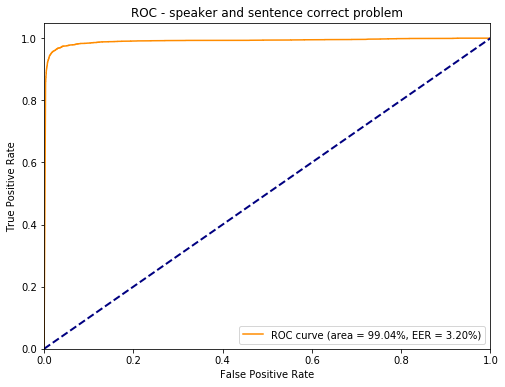
\includegraphics[width=0.8\textwidth]{images/2_2_b_roc_example}
    \caption{Przykładowy wykres krzywej \shortcut{ROC} wygenerowany na podstawie wyników modelu \shortcut{GMM-UBM} opisanego w~pracy}
    \label{fig:2_2_b_roc_example}
\end{figure}

\subsection{Long Short-Term Memory}

Rekurencyjne sieci neuronowe (\shortcut{RNN}, \foreign{Recursive Neural Network}) to rodzaj sieci neuronowych,
które, jak \shortcut{HMM}, służą do modelowania ciągów obserwacji w~czasie. Posiadają one połączenia między
ukrytymi warstwami, które prowadzą do tej samej lub poprzednich warstw
(w przeciwieństwie do sieci \foreign{feed-forward}) i~przekazują wartości z~opóźnieniem
w czasie\cite{onTheDifficulty}.

Choć prosta architektura, w~której wyjścia z~warstwy są ponownie przekazywane na jej wejście, pozwala
wyrazić wiele zależności, to wyznaczenie parametrów w~tej sieci sprawia trudności. Jeżeli zamiast
ręcznie dobierać wagi zastosuje się do ich wyznaczenia metodę gradientową, pojawia się problem
z zanikającym lub eksplodującym gradientem. Polega on na tym, iż przy liczeniu gradientu błędu
następuje wielokrotne mnożenie przez macierz wag. Jeżeli ta operacja powoduje zmianę długości
wektora, to przy wielokrotnym mnożeniu ta długość szybko będzie rosnąć lub maleć. Sprawia to,
że trudno jest odpowiednio dopasować wagi, gdy wynik zależy od ramki w~odległej przeszłości.

W \shortcut{LSTM} ten problem został ominięty. W~ich przypadku poza tym, że wartości na wyjściu są przekazywane
na wejście w~następnej chwili czasu, na stan składa się także dodatkowa komórka z~ukrytym stanem.
Architektura sieci jest tak wymyślona, że stan ukryty jest mnożony tylko przez bramkę o~ograniczonych wartościach
oraz w~sumowany z~nowym kandydatem na stan ukryty, lecz nie jest wielokrotnie mnożony przez żadną macierz o
trudnej do ograniczenia postaci. Może zatem zostać w~pewnej części wymazany lub zastąpiony, lecz jego długość
nie ma tendencji, by z~każdym krokiem wykładniczo rosnąć lub maleć. Tak samo przy liczeniu gradientu
zachowywana jest jego długość. Utrzymywanie takiej samej wartości stanu ukrytego przez wiele kroków lub
jego całkowite zastąpienie w~jednym kroku jest proste do osiągnięcia.

W poniższych wzorach $\cdot$ oznacza iloczyn macierz-wektor, a~$\circ$ operację wymnożenia parami
elementów wektorów równej długości. Pojedynczy neuron sieci \shortcut{LSTM} opisuje się tak:

\begin{align*}
& x_t & \text{wejście w~chwili } t\\
& X_t = [h_{t-1}, x_t] & \text{konkatenacja } x_t \text{ i~} h_t\\
& f_t = \sigma(W_f \cdot X_t + b_f) & \text{bramka zapomnienia}\\
& i_t = \sigma(W_i \cdot X_t + b_i) & \text{bramka wejścia}\\
& o_t = \sigma(W_o \cdot X_t + b_o) & \text{bramka wyjścia}\\
& \bar{C_t} = tanh(W_c \cdot X_t + b_c) & \text{nowy kandydat na stan}\\
& C_t = f_t \circ C_{t-1} + i_t \circ \bar{C_t} & \text{nowy ukryty stan komórki}\\
& h_t = o_t \circ tanh(C_t) & \text{wyjście w~chwili } t
\end{align*}

\begin{figure}[H]
    \centering
    \begin{tikzpicture}[->, >=stealth',shorten >=1pt,auto,very thick,node distance=2cm]
        \tikzset{VertexStyle/.style = {
                draw,
                shape          = circle,
                color          = blue,
                text           = black,
                inner sep      = 2pt,
                outer sep      = 0pt,
                minimum size   = 1.25cm,
                font=\Large\bfseries
        }}
        \tikzset{EdgeStyle/.style   = {
        }}

        \node[VertexStyle](Ct1){$C_{t-1}$};
        \node[VertexStyle,right=of Ct1](xt){$[h_{t-1}, x_t]$};
        \node[VertexStyle,above=of xt](it){$i_t$};
        \node[VertexStyle,left=of it](ft){$f_t$};
        \node[VertexStyle,right=of it](bCt){$\bar{C_t}$};
        \node[VertexStyle,right=of bCt](ot){$o_t$};
        \node[VertexStyle,above=of it](ht){$h_t$};
        \node[VertexStyle,left=2.75cm of ht](Ct){$C_t$};

        \draw[EdgeStyle,bend left=20](xt) to node{} (ft);
        \draw[EdgeStyle](xt) to node{} (it);
        \draw[EdgeStyle,bend right=20](xt) to node{} (bCt);
        \draw[EdgeStyle,bend right=20](xt) to node{} (ot);
        \draw[EdgeStyle](ft) to node{} (Ct);
        \draw[EdgeStyle,bend right=20](it) to node{} (Ct);
        \draw[EdgeStyle,bend right=15](bCt) to node{} (Ct);
        \draw[EdgeStyle,bend right=20](ot) to node{} (ht);
        \draw[EdgeStyle](Ct) to node{} (ht);
        \draw[EdgeStyle,bend left=20](Ct1) to node{} (Ct);
    \end{tikzpicture}
    \caption{Graf przedstawiający zależności w~opisie LSTM}
    \label{fig:2_2_lstm_graph}
\end{figure}

Parametrami są wagi przy bramce zapomnienia $W_f$ i~$b_f$, wagi przy bramce wejścia $W_i$, $b_i$, wagi przy bramce wyjścia $W_o$, $b_0$, wagi, którymi generowany jeset nowy kandydat na stan $W_c$, $b_c$. Jeżeli wektor wejściowy $x_t$ ma rozmiar $N$, a~stan ukryty $C_t$ oraz wyjście sieci $h_t$ to wektory rozmiaru $M$, to $X_t$ ma rozmiar $M + N$, wyjścia na czterech bramkach mają rozmiar $M$. Macierze parametrów na bramkach mają rozmiar $M + N \times M$ oraz $M$. Sieć można wytrenować z~użyciem
wstecznej propagacji w~czasie\cite{longShortTerm}.

\section{Istniejące systemy weryfikacji mówcy}\label{sec:istniejace_systemy}

\subsection{Metody niezależne od tekstu}

Jednym ze sposobów weryfikacji mówcy stosowanym od dawna jest \shortcut{GMM-UBM}. Polega on na utworzeniu modelu tła
(\foreign{universal background model}), modelu mikstur gaussowskich i~dopasowaniu ich do ramek \shortcut{MFCC} z~nagrań
treningowych. Dla każdego mówcy tworzony jest osobny model przez \shortcut{MAP}-adaptację modelu tła do nagrań danego
mówcy. W~\cite{utteranceVerificationFor}
następnie liczona jest różnica między logarytmem prawdopodobieństwa wygenerowania nagrania przez model
dla mówcy i~przez model tła. Różnica ta porównywana jest z~progiem i~na tej podstawie podejmowana jest decyzja
o weryfikacji. Podobnie można weryfikować treść nagrania, przez adaptację modelu tła do nagrań konkretnej treści.
Jeżeli treść wszystkich wypowiedzi jest znana i~jest to zbiór zamknięty, to zamiast porównywać model dla jednej
treści z~modelem tła, można wykorzystać \foreign{mean norm} lub \foreign{max norm}, to znaczy porównać wynik weryfikowanego
modelu ze średnim wynikiem pozostałych lub z~najlepszym wynikiem pozostałych. Niezależnie weryfikowany jest mówca
i treść wypowiedzi.

Autorzy testują wiele modeli, w~tym zarówno do weryfikacji mówcy, jak i~treści wykorzystują \shortcut{GMM-UBM} z~512 miksturami.
Jako cech używają 19 \shortcut{MFCC} z~delta i~delta-delta cechami. \shortcut{MAP}-adaptację przeprowadzono
z parametrem \foreign{relevance factor} 3.
Do weryfikacji mówcy przy adaptacji korzystają z~nagrań tego mówcy, a~do weryfikacji treści nagrań tej samej treści.

Podejście z~miksturami można rozwinąć. Bardzo popularnym rozwinięciem są i-wektory, w~których
zamiast liczyć log-prawdopodobieństwo liczone są wektory charakteryzujące mówcę, a~następnie do
odpowiedzenia na problem weryfikacji wykorzystywane
jest \shortcut{LDA} (\foreign{Linear Discriminant Analysis}), które jest metodą nadzorowanego klastrowania.

Na przykład w~\cite{utteranceVerificationFor}
zastosowano i-wektory do weryfikacji mówcy. Trenują \shortcut{GMM-UBM} z~512 miksturami, osobno dla każdej płci.
I-wektor ma rozmiar 400, i-wektor dla danego mówcy jest średnią z~wszystkich i-wektorów dla jego nagrań.
Długość i-wektorów jest następnie normalizowana. Do weryfikacji użyta jest \shortcut{gPLDA}.
(\foreign{gaussian probabilistic linear discriminant analysis})

%%% GMM i-vectors JFA

\subsection{Metody zależne od tekstu}

Powyższe systemy nie uwzględniają kolejności w~jakiej ramki powinny być w~wypowiedzi. W~problemie weryfikacji
zależnej od tekstu jest to jednak możliwe i~powinno pozwolić na poprawienie skuteczności systemu.
W \shortcut{GMM-UBM} te same mikstury uczestniczą niezależnie od czasu, a~i-wektory są uśredniane dla całej
wypowiedzi. Na szczęście dzięki użyciu \shortcut{HMM} lub \shortcut{DTW} możliwe jest uwzględnienie tych
informacji\cite{parallelSpeakerAnd}.

W pracy \cite{parallelSpeakerAnd}
pracy utworzono kilka modeli \shortcut{HMM} z~emisjami \shortcut{GMM}. Autorzy osobno
zajmują się problemem weryfikacji mówcy i~weryfikacji treści. Używany jest zbiór \techname{RedDots}.

Najpierw tworzony jest tam \shortcut{HMM} dla każdej frazy w~ten sposób, że emisje modelu są inicjalizowane przez
skopiowanie parametrów \shortcut{UBM},
a następnie dotrenowane z~użyciem wszystkich nagrań treningowych z~pewnym zdaniem.
Następnie dla każdego mówcy model danego zdania jest kopiowany i~MAP-adaptowany do jego nagrań tego zdania.
Przy weryfikacji mówcy za pomocą algorytmu Viterbiego obliczany jest logarytm
prawdopodobieństwa, że nagranie pochodzi od danego mówcy oraz że nagranie pochodzi od \shortcut{HMM} tła.
Ocena nagrania to różnica między tymi wynikami i~system decyduje o~weryfikacji porównując tę różnicę z~pewnym progiem.

Następnie tworzą drugi podsystem do weryfikacji treści. Dzielą nagrania tej samej frazy na pewną liczbę segmentów
i tworzą dla każdej frazy \shortcut{HMM} typu \foreign{left-to-right}. Jako, że nagrań jest mało, to trudno
wytrenować model, by był w~stanie wykryć, które ramki zawierają jakie fony, dlatego segmenty dzielą na sztywno
i właściwie ręcznie dopasowują mikstury do ramek. Weryfikacja frazy przebiega w~ten sposób, że liczą średnią
różnicę w~log-prawdopodobieństwie między pochodzeniem frazy z~odpowiedniej dla mówcy i~segmentu mikstury, a
pochodzeniem ramki z~\shortcut{GMM-UBM}, zamiast \shortcut{HMM}.

Użyli 19 \shortcut{MFCC} z~delta i~delta-delta cechami. \shortcut{GMM-UBM} ma 512 mikstur. \shortcut{MAP} adaptacja
dotyczy tylko wektora średnich. Liczba segmentów w~drugiej części to 4 i~8, lecz 8 nie poprawiło im wyników. Liczba
stanów HMM w~pierwszej części to 4 lub 8 i~8 lekko poprawiło im wyniki.

Podobny pomysł jest wykorzystany w~jednym z~systemów do weryfikacji treści w~\cite{utteranceVerificationFor}, gdzie
autorzy wytrenowali 512 miksturowy \shortcut{GMM UBM}. Ich HMM jest typu \foreign{left-to-right} z~5 stanami.
Naukę rozpoczynają dzieląc jedno nagranie na 5 równych segmentów.
Każdy z~5 \shortcut{GMM} emitujących \shortcut{MAP}-adaptują z~modelu tła korzystając z~próbek odpowiedniego segmentu.
Pozostałe nagrania są dzielone na segmenty korzystając z~tego modelu. Następnie trenują ostateczne modele dla każdej
wypowiedzi \shortcut{MAP}-adaptując model tła korzystając z~wszystkich nagrań, zakładając podział na ramki jak
w poprzednim kroku.

W \cite{comparisonOfMultiple}
model \shortcut{HMM} został bardziej rozwinięty. Wykorzystano wiedzę o~treści wypowiedzi w~postaci transkrypcji.
Mając transkrypcje można stworzyć i~dopasować wiele \shortcut{GMM} do rozpoznawania różnych głosek, zamiast
używać jednej mikstury z~bardzo dużą liczbą elementów. Można wykorzystać model stworzony na potrzeby rozpoznawania mowy.
Taki model ma stany ukryte, które mają odpowiadać fonemom języka. Na przykład angielski ma 39
fonemów, czemu odpowiadałoby 39 stanów, lecz powszechne jest rozszerzenie
modelu do 3 stanów na jeden fonem, co ma pozwolić osobno określić cechy dla początku, środka i~końca fonemu.
Bardziej złożone systemy, jak \shortcut{HTK}\cite{theHtkBook}
, dodatkowo pozwalają na zbudowanie tzw. modelu trójfonowego (\foreign{triphone}), co oznacza,
że nie używają trzech stanów na fonem, lecz
przypisują inne stany w~zależności od fonemu bezpośrednio przed i~bezpośrednio po danym fonemie.
Powoduje to duży wzrost wymaganych stanów, to znaczy z~$3 \times 39$ do $3 \times 39^3$,
dlatego te systemy dodatkowo łączą bardzo podobne trójki, by dzieliły ze sobą mikstury.
Określenie podobieństwo bazuje na wiedzy o~podziałach głosek i~tym jak układ głosowy przechodzi między nimi.
W \cite{comparisonOfMultiple}
użyto modelu jednofonowego (\foreign{monophone}), choć użyli też trójfonowego w~nieco innym przypadku.

Do modelowania emisji używa się \shortcut{GMM}. Jako, że stanów jest dużo więcej niż w~\shortcut{GMM-UBM}
lub w~\shortcut{HMM}, w~którym wypowiedź jest podzielona na 4-5 części, to
w opisanym przykładzie tego modelu zastosowane jest 8 mikstur zamiast 512 lub 1024. Wyjątkiem są ramki,
gdzie spodziewana jest cisza (początek, koniec i~przerwa między wyrazami), tam
użyto 16 mikstur. Warto zauważyć, że we front-endzie użyto 20 \shortcut{MFCC} wziętych z~banku filtrów rozmiaru
40 i~dołączono cechy delta i~delta-delta.

Mając taki model można użyć algorytmu Viterbiego lub \foreign{forward-backward}, by przypisać ramkom z~nagrania
fonemy, które na nich występują. Dla każdego mówcy
przez \shortcut{MAP}-adaptację można stworzyć ich własny zestaw mikstur do każdego stanu i~potem weryfikować
mówcę przez porównanie logarytmu prawdopodobieństwa
pochodzenia nagrania od mówcy, a~pochodzenia od modelu do rozpoznawania mowy, tak jak
w opisanej wcześniej \shortcut{GMM-UBM}.

Zamiast tego na przykład w~tej pracy \cite{iVectorHmmBased}
użyto \shortcut{HMM}, lecz dokonując rejestracji i~weryfikacji z~wykorzystaniem metody i-wektorów.
W przeciwieństwie do poprzedniej pracy, tu \shortcut{HMM} jest jednofonowy. Autorzy przetestowali
i-wektory rozmiaru 400 oraz 600 i~dokonują weryfikacji przez obliczenie podobieństwa cosinusowego.

\subsection{Metody wykorzystujące sieci neuronowe}

W \cite{aNovelSchemeFor}
połączono ideę i-wektorów z~\shortcut{DNN}. Autorzy zauważyli, że do obliczenia i-wektorów można użyć
dowolnego modelu, który definiuje $K$ klas i~pozwala obliczyć prawdopodobieństwo
przynależności do klasy dla ramki $P(\theta_k | x)$.
Tutaj użyto \shortcut{DNN} wytrenowanej na nagraniach z~transkrypcją do rozpoznawania mowy.
Sieć ma 7 warstw, 1200 wymiarów w~warstwach ukrytych, w~ostatniej warstwie ma 3450 wymiarów i~funkcję aktywacji softmax.
Wyjścia interpretowane są jako przynależności do trójek fonów. Trójki te pełnią rolę klas,
a wartość na wyjściu traktowane są jako wymagane prawdopodobieństwo, dzięki czemu \shortcut{DNN}
może zastąpić \shortcut{GMM}
przy obliczaniu statystyk w~metodzie i-wektorów. Weryfikacja następuje z~wykorzystaniem \shortcut{gPLDA}.

W \cite{timeDelayDeep}
również użyta została \shortcut{DNN} do rozpoznawania mowy i~zaadaptowana do weryfikacji mówcy.
Wykorzystana sieć ma architekturę \shortcut{TDNN} (\foreign{Time-delay neural network}). Ma 6 warstw \foreign{feed-forward},
na wejściu przyjmuje kilka kopii sygnału wejściowego z~różnym przesunięciem w~czasie, wagi
w warstwach przetwarzających kopie są współdzielone. Takie przetwarzanie kilku kopii jest wykonywane na
4 warstwach, z~różnym przesunięciem i~w~efekcie sieć ma uwzględniać kontekst aż 13 ramek
z przeszłości i~9 ramek z~przyszłości. Ostatnia warstwa kończy się softmaxem z~wyjściami odpowiadającymi 5297 trójkom fonemów.
Ciekawe są następne kroki autorów, gdyż trenują \shortcut{GMM} rozmiaru również 5297
i dopasowują mikstury w~ten sposób, że dla $k$-tej mikstury estymują jej wektor średnich i~macierz kowariancji (pełną)
do danych ważonych przynależnością do $k$-tej trójki fonemów wyznaczoną przez \shortcut{TDNN}.
Następnie używają \shortcut{GMM} standardowo do i-wektorów (600 wymiarowych) i~\shortcut{PLDA}.
Autorzy zauważają również, że sieć i~\shortcut{GMM} mogą używać różnych wektorów cech,
co może być korzystne, gdyż rozwiązują różne problemy - klasyfikacji fonemów oraz weryfikacji mówcy.

W \cite{investigationOfBottleneck}
używany jest \shortcut{DNN} wytrenowany do rozpoznawania fonemów. Najpierw autorzy wytrenowali
\shortcut{GMM-HMM}, by wykorzystać go do przypisywania do ramek sygnału jaki
jest w~nich fonem. Następnie na tych danych, tym razem już oznakowanych przez \shortcut{GMM-HMM},
trenowany jest \shortcut{DNN} do dyskryminacji fonemów. Autorzy używają
jednocześnie nagrań z~angielskiego i~chińskiego, by rozpoznawać więcej fonemów i~uzyskać model działający
dla wypowiedzi w~różnych językach.
Sieć jest wykorzystywana w~roli ekstraktora cech. Wektor wartości na wyjściu przedostatniej warstwy
tej sieci jest wykorzystywany jako tzw. \foreign{bottleneck features}.
Warstwa ta ma nieco mniej neuronów, by uzyskać tam niskowymiarową reprezentację ramek na wejściu.
Jako, że sieć została wytrenowana do rozpoznawania fonemów, to cechy te powinny
wydajnie uwzględniać informację niezbędne właśnie do tego celu, choć nie jest jasne, czemu miałyby być
tam informacje charakteryzujące mówcę.
\shortcut{GMM} są trenowane na tych cechach, tak jak w~innych systemach są trenowane na \shortcut{MFCC}
i używane do ekstrakcji i-wektorów. Weryfikacja następuje przez \shortcut{gPLDA}.

Zaletą \shortcut{DNN} jest możliwość operowania na większych wektorach, dlatego na wejściu sieć otrzymuje
oprócz jednej ramki też po 5 ramek sąsiadujących przed i~po, łącznie 11,
do tego każda ramka zawiera 40 współczynników z~filtrów w~częstotliwości melowej oraz 80 cech delta i~delta-delta.
Sieć ma pięć warstw ukrytych, wszystkie mają wyjścia rozmiaru 1200, z~wyjątkiem
ostatniej, która ma rozmiar 39 i~generuje \foreign{bottleneck features}. Na wyjściu autorzy rozważają
różny rozmiar wektora, jednak wszystkie rozważone parametry są ponad 2000 i~są zależne
od budowy \shortcut{HMM-GMM} i~tego ile trójek fonemów rozróżnia. Tworzone później
\shortcut{GMM} ma 2048 mikstur, i-wektory są rozmiaru 400, \shortcut{gPLDA} operuje w~200 wymiarach.
Warto zauważyć, że ostateczny wynik osiągnięty przez autorów ma wyższą \shortcut{EER} niż \foreign{baseline}
w postaci \shortcut{GMM-UBM}.

W pracy \cite{endToEnd} opisany jest model stworzony przez Google do weryfikacji mówcy. Wszystkie wykorzystane
w nim nagrania zawierały fazę "Ok Google", a~zatem zbiór ten jest uboższy wobec poprzednio wymienionych rozwiązań.
Zaproponowane modele, bazujące na sieci neuronowej, charakteryzują się tym, że w~całości rozwiązują problem weryfikacji
i są trenowane w~całości, podczas gdy poprzednio wymienione modele były rozbite na osobno działające podsystemy.
Na przykład \shortcut{DNN} z~poprzednich prac były trenowane do rozpoznawania mowy i~zaadaptowane do rozpoznawania
mówcy albo w~przypadku \shortcut{GMM} celem jest modelowanie dystrybucji cech, nie weryfikacja. Takie rozbicie
skutkuje nieoptymalnym działaniem i~zwiększa złożoność obliczeń.

Pierwsza sieć, którą zaproponowali autorzy, to \shortcut{DNN} z~lokalnie połączoną pierwszą warstwą i~w~pełni połączonymi
kolejnymi warstwami. Warstwy używają funkcji aktywacji \shortcut{ReLU}, z~wyjątkiem
ostatniej z~\foreign{softmaxem}. Wektor na wyjściu ma wymiar na każdego mówcę. Po wytrenowaniu sieci, dla każdej
ramki z~nagrania obliczane są wartości na wyjściach ostatniej ukrytej warstwy,
są one uśredniane dla nagrania i~wynik nazywany jest d-wektorem. Pierwszy system działa przez obliczenie d-wektora
na nagraniach rejestracyjnych i~uśrednieniu, by uzyskać d-wektor opisujący mówcę.
Dla nagrań testowych również jest liczony d-wektor i~weryfikacja następuje przez obliczenie cosinusowego podobieństwa
między tym d-wektorem i~d-wektorem mówcy. Warto zauważyć, że w~przeciwieństwie
do \foreign{bottleneck features}, tutaj sieć do ekstrakcji cech jest wytrenowana do rozpoznawania mówców, a~nie
fonemów, więc można się spodziewać, że zachowuje informacje charakteryzujące mówcę.
Przy \foreign{bottleneck features} można podejrzewać, że cechy mówców są wręcz odrzucane, gdyż w~problemie
rozpoznania fonemów są przeszkodą.

Druga sieć przyjmuje nagranie testowe oraz kilka nagrań rejestracyjnych i~zwraca na wyjściu jedną liczbę
reprezentującą wynik weryfikacji. Sieć ma architekturę \shortcut{LSTM}. Brane pod uwagę
jest tylko wyjście sieci dla ostatniej ramki nagrania, przy czym jako, że to sieć rekurencyjna,
to wynik może zależeć od wszystkich ramek poprzedzających. Reprezentacja mówcy jest tworzona przez uśrednienie
wyjścia \shortcut{LSTM} dla nagrań rejestracyjnych. Nagrania testowe również przechodzą przez sieć i~są
porównywane z~reprezentacjami mówców przez obliczenie podobieństwa cosinusowego. Autorzy raportują, że dopiero
dla bardzo dużej liczby danych to rozwiązanie osiągnęło wysoką skuteczność.

